
\chapter{Kombinatorik}

\section{Endliche Summen}
\subsection{Definition}

\begin{Definition}[Summe]\index{Summe}
Für eine Folge $a\colon\N\to\R$ ist die Summe über die $a_k$
von $k=m$ bis $n$ rekursiv definiert gemäß%
\[
\sum_{k=m}^{m-1} a_k := 0,\qquad
\sum_{k=m}^n a_k := a_n+\sum_{k=m}^{n-1} a_k.
\]
\end{Definition}
Das schaut komplizierter aus als es ist. Man hat
\[\sum_{k=1}^n a_k = a_1+a_2+a_3+\ldots+a_n.\]
Z.\,B. ist
\[\sum_{k=1}^4 k^2 = 1^2+2^2+3^2+4^2 = 1+4+9+16 = 30.\]
Die Berechnung gemäß der Definition:
\begin{align*}
\sum_{k=1}^4 k^2 &= 4^2+\sum_{k=1}^3 k^2
= 4^2+3^2+\sum_{k=1}^2 k^2
= 4^2+3^2+2^2+\sum_{k=1}^1 k^2\\
&= 4^2+3^2+2^2+1^2+\sum_{k=1}^{0} k^2 = 4^2+3^2+2^2+1^2+0 = 30.
\end{align*}

\subsection{Rechenregeln}
\begin{Satz}[Homogenität der Summenoperation]%
\index{Homogenität}
Ist $c$ eine Konstante, dann gilt
\[\sum_{k=m}^n ca_k = c\sum_{k=m}^n a_k.\]
\end{Satz}
\strong{Beweis.}
Der Induktionsanfang ist trivial:
\[\sum_{k=m}^{m-1} ca_k = 0 = c\cdot 0 = c\sum_{k=m}^{m-1} a_k.\]
Der Induktionsschritt »$A(n-1)\Rightarrow A(n)$« ist erfüllt, denn es gilt
\[\sum_{k=m}^n ca_k = ca_n+\sum_{k=m}^{n-1} ca_k = ca_n+c\sum_{k=m}^{n-1} a_k
= c\bigg(a_n+\sum_{k=m}^{n-1} a_k\bigg) = c\sum_{k=m}^n a_k.\;\qedsymbol\]

\section{Permutationen}%
\index{Permutation}

\subsection{Anzahl der Permutationen}

Gegeben sind zwei unterschiedliche Buchstaben, sagen wir $A,B$. Diese
Buchstaben sind auf zwei Plätze zu legen, wobei die Reihenfolge die
wesentliche Rolle spielt. Wie viele Möglichkeiten gibt es dafür?
Das sind zwei, nämlich $AB$ und $BA$. Man sagt, es gibt zwei
Permutationen der Buchstaben $A,B$.

Wie viele Möglichkeiten gibt es, die drei Buchstaben $A,B,C$ auf
drei Plätze zu legen? Es sind sechs, das sind
$ABC$, $BAC$, $ACB$, $BCA$, $CAB$ und $CBA$. Man sagt, es gibt
sechs Permutationen der Buchstaben $A,B,C$.

Das ist schon recht unübersichtlich. Es gibt aber eine systematische
Methode, alle Möglichkeiten aufzuzählen. Für den ersten Platz gibt
es drei Möglichkeiten. Für den zweiten Platz gibt es dann jeweils
nur noch zwei Möglichkeiten, weil nur noch zwei Buchstaben zur
Verfügung stehen. Für den letzten Platz bleibt jeweils eine
Möglichkeit. Somit ergibt sich die folgende Baumstruktur:

\begin{figure}[h]
\begin{center}
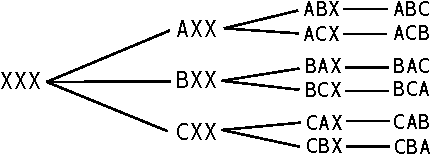
\includegraphics[width=0.5\textwidth]{img/Perm-ABC.pdf}
\end{center}
\end{figure}

\noindent
Gegeben sind nun $n$ Buchstaben und genau so viele freie Plätze.
Die Anzahl der Permutationen nennen wir $n!$, sprich \emph{$n$ Fakultät}.
Für den ersten Platz gibt es $n$ Möglichkeiten. Für den zweiten Platz
sind nur noch jeweils $n-1$ Buchstaben übrig, es gibt deshalb nur noch
jeweils $n-1$ Möglichkeiten. Für den dritten Platz gibt es noch jeweils
$n-2$ Möglichkeiten, für den vierten Platz jeweils $n-3$ usw. Für den
$n$-ten Platz gibt es schließlich jeweils nur noch eine Möglichkeit.
Das macht insgesamt
\[n! = n\cdot (n-1)\cdot (n-2)\cdot\ldots\cdot 3\cdot 2\cdot 1\]
Möglichkeiten. Außerdem ergibt sich die folgende Rekursionsformel:
\[n! = n\cdot (n-1)!.\]
\begin{Definition}[Fakultät]\index{Fakultät}
Für eine Zahl $n\in\N_0$ ist die Fakultät von $n$ rekursiv
definiert gemäß
\[0! := 1,\qquad n! := n\cdot (n-1)!.\]
\end{Definition}
Wir zuvor gezeigt, gibt es genau $n!$ Permutationen von $n$
unterschiedlichen Objekten. Es gibt $4!=24$ Permutationen
der vier Buchstaben $A,B,C,D$, aber schon $5!=120$ Permutationen der
fünf Buchstaben $A,B,C,D,E$. Die Anzahl der Permutationen wächst
rasant. Es gibt z.\,B. unzählige Möglichkeiten, Bücher in ein
längeres Buchregel zu stellen.

